%!TEX program = xelatex
\documentclass[10pt,handout]{beamer}
% \documentclass[10pt]{beamer}

\usetheme[progressbar=frametitle]{metropolis}
\usepackage{appendixnumberbeamer}

\usepackage{fontspec}
\setmainfont{Libertinus Sans}
\setsansfont{Libertinus Sans}

\usepackage{booktabs}
\usepackage{array}
\newcolumntype{P}[1]{>{\raggedright\arraybackslash}p{#1}}
\usepackage{longtable}
\usepackage{amsmath}
\usepackage{multirow}
\usepackage{adjustbox}
\usepackage{qrcode}
\usepackage{graphicx}
\usepackage{subfig}
\usepackage{dcolumn} 
\usepackage{threeparttable} 
%\usepackage{showframe} 

% Setting the paths for graphics:
% ../Figures/ ([root]/Figures) for plots generated in R
%  ./Diagrams/ ([root]/Presentation/Diagrams) for diagrams 
\graphicspath{{..}{../Figures/}{./Diagrams/}{./Figures/}{./Diagrams}} 

% Animations made from split .pdfs, stored in ./Diagrams/*
\usepackage{animate} 

\title{Regional telework}
\subtitle{\small Regional perspective of labour market change during and after COVID-19}
\date{22 May 2023}
\author{Matteo Sostero} 


\begin{document}
\metroset{block=fill}
\maketitle

\begin{frame}{Outline}
Present exploratory and descriptive analysis of EU Labour Force Survey (EU LFS) micro-data by:
\begin{itemize}
  \item country, regions (NUTS 1-2)
  \item degree of urbanisation of respondent's residence (degurba): \emph{Cities, Towns and suburbs, Rural areas}
  \item type of region (urbrur): \emph{Capital region, Mainly urban, Intermediate, Mainly rural, Undifferentiated}
  \item regional connectivity statistics
  \item occupation (ISCO 1, 2, or 3 digits)
  \item housekeeping/harmonisation
\end{itemize}
\end{frame}

\section{Change in telework by countries and regions}

\begin{frame}{Telework index by region}
\centering
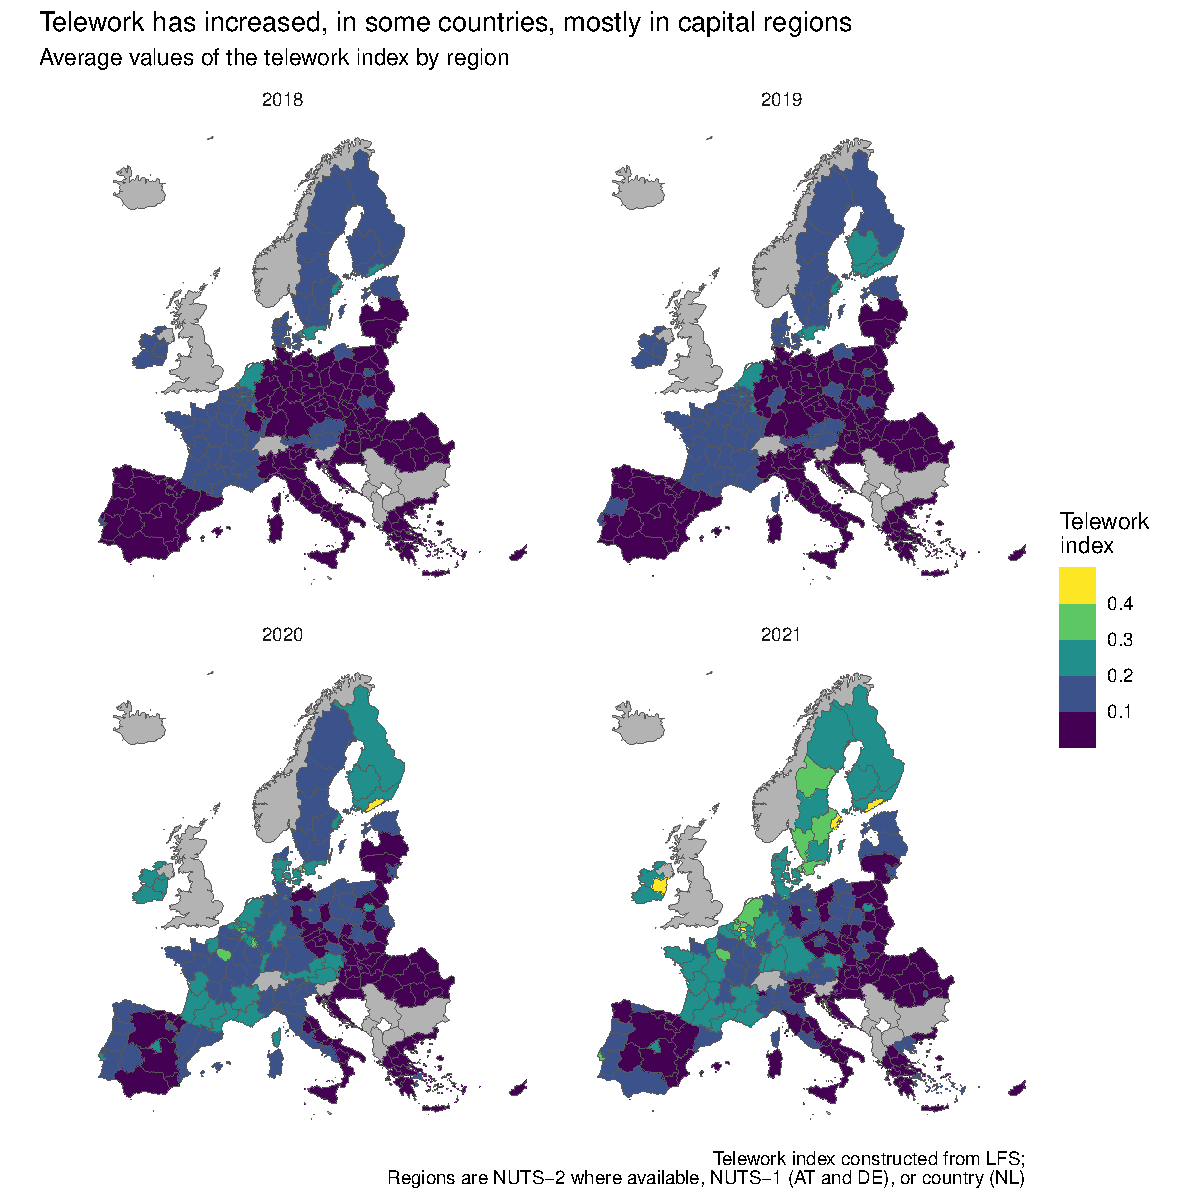
\includegraphics[width=\textwidth,height=0.85\textheight,keepaspectratio]{Telework_nuts_years.pdf}

Interactive: \url{https://rpubs.com/m-sostero/hwi}
\end{frame}

\begin{frame}{Change in telework index by countries and regions}
\centering
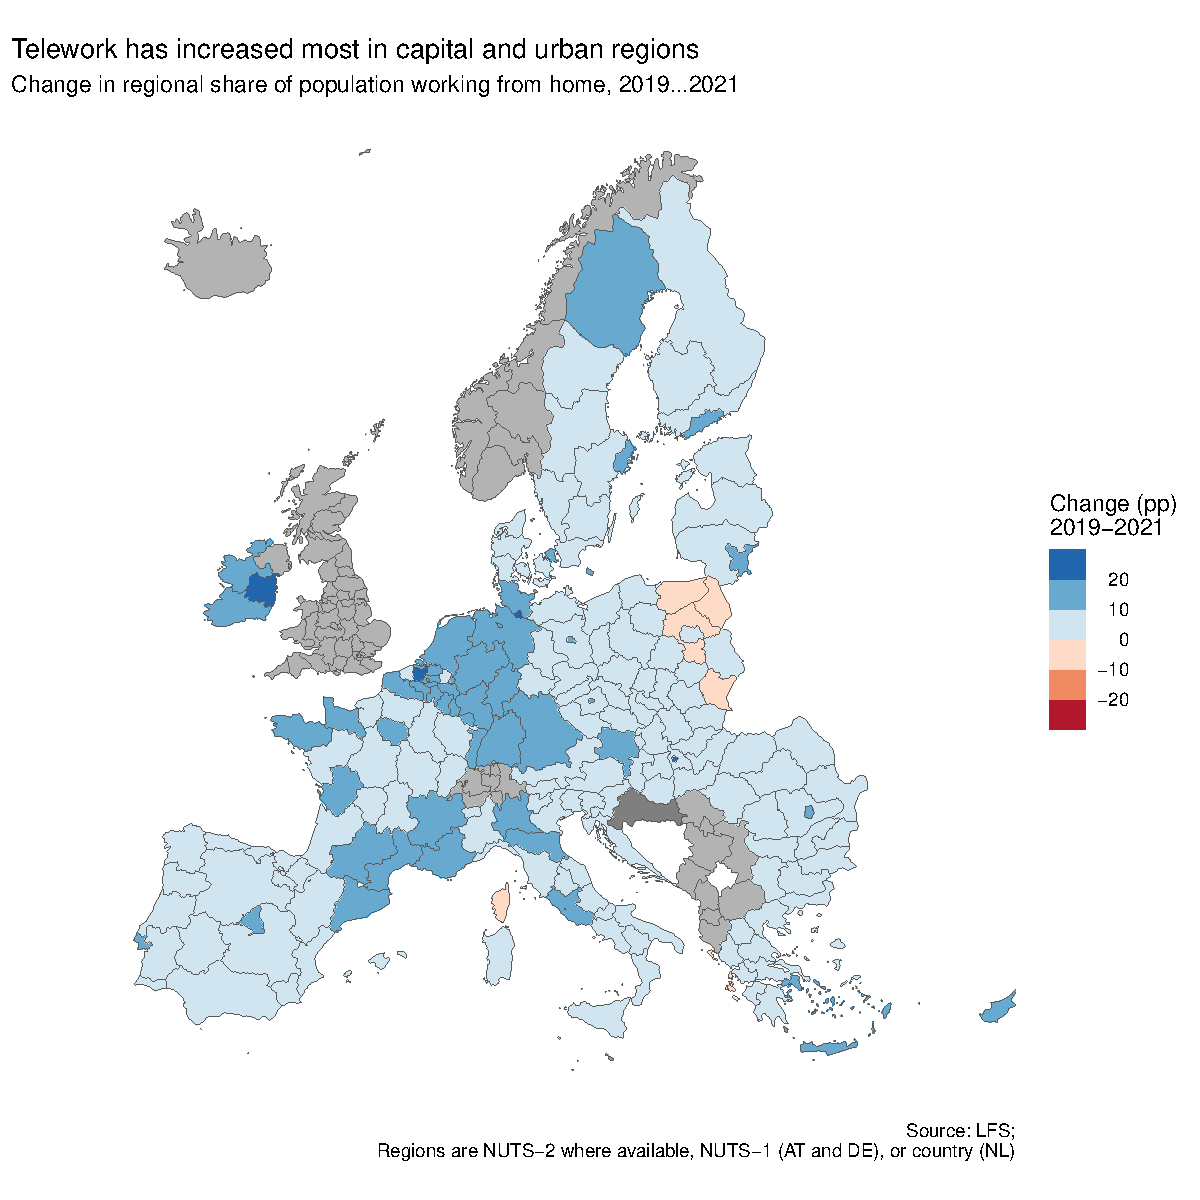
\includegraphics[width=\textwidth,height=0.9\textheight,keepaspectratio]{Telework_nuts_change.pdf}
\end{frame}

\begin{frame}{Change in telework index by countries and regions}
Interpretation:
\begin{itemize}
\item Marked changes in overall telework frequency (as measured from LFS) relative to before COVID
\item Significant variation \emph{across} countries (country fixed-effect).
\item Variation \emph{within} countries, in terms of capitals/urban regions vs the rest?
 \end{itemize}
\end{frame}

\section{Degree of urbanisation}
\begin{frame}{Telework index by degurba}
\pause
\centering
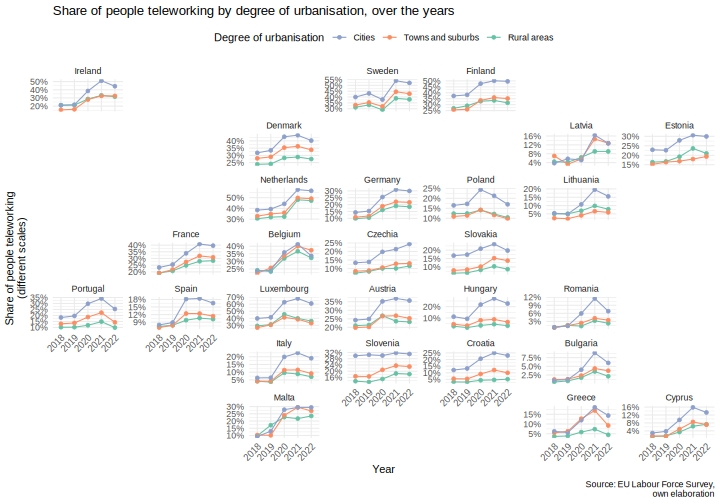
\includegraphics[width=\textwidth,height=0.9\textheight,keepaspectratio]{Telework_degurba_eu.pdf}
\end{frame}

\begin{frame}{Telework index by degurba, selected countries }
\pause
\centering
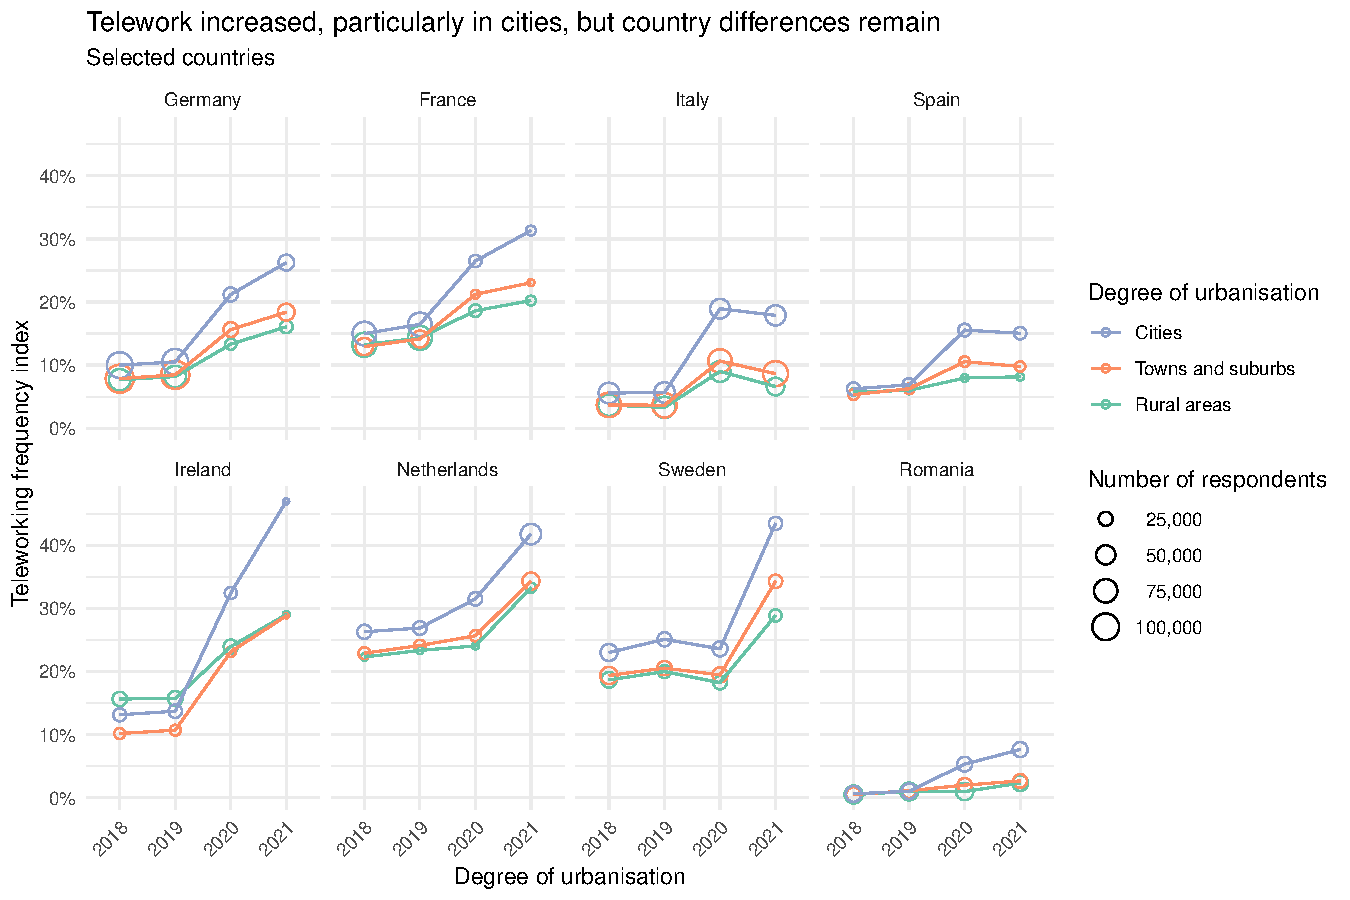
\includegraphics[width=\textwidth,height=0.9\textheight,keepaspectratio]{Telework_degurba_selected.pdf}

Interactive: \url{https://rpubs.com/m-sostero/hw\_degurba}
\end{frame}

\begin{frame}{Changes in telework: cities vs rural areas}
\pause
\centering
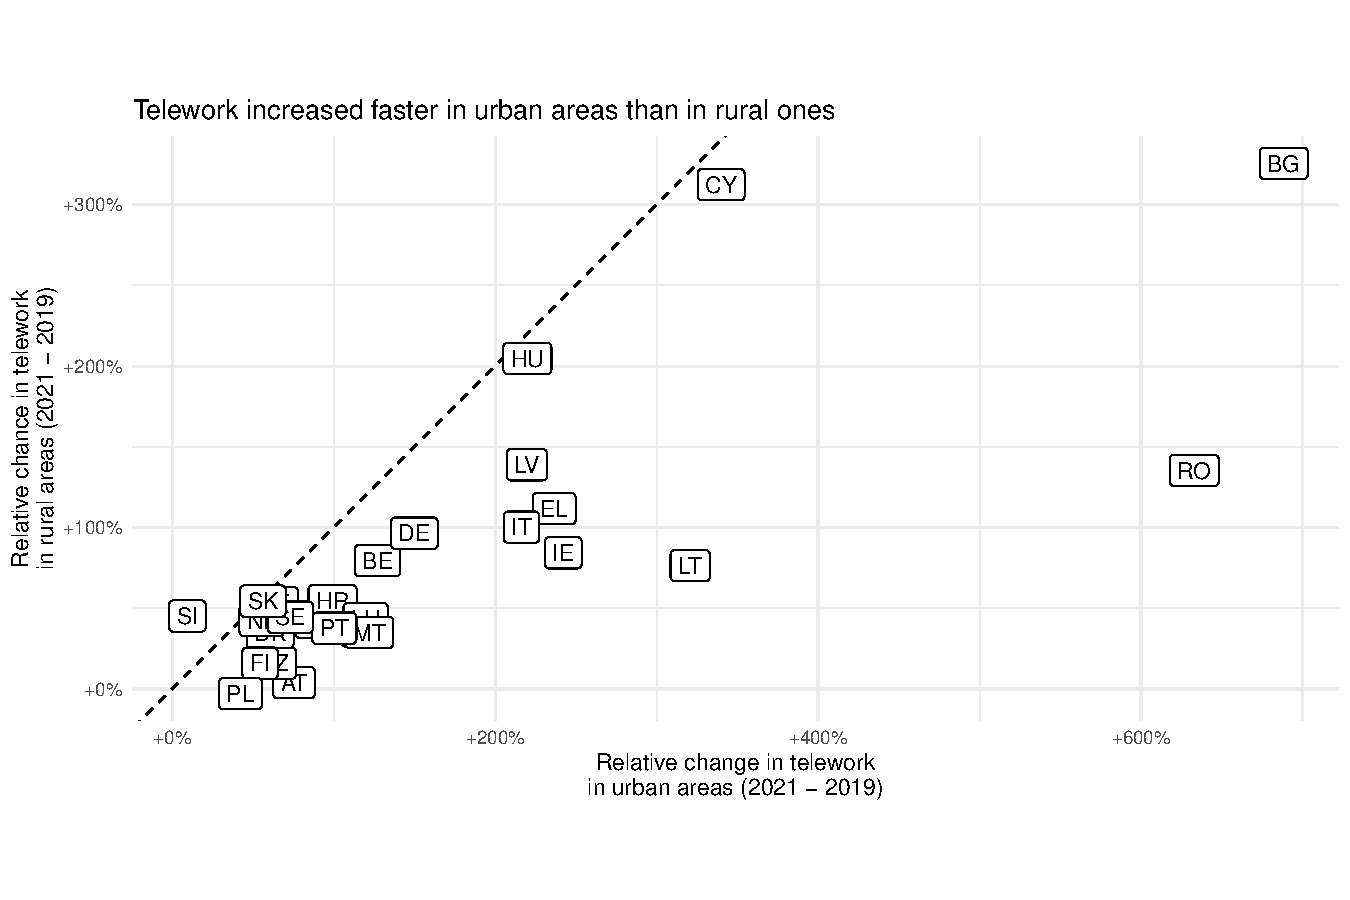
\includegraphics[width=\textwidth,height=0.9\textheight,keepaspectratio]{Telework_changes_degurba.pdf}
\end{frame}

\begin{frame}{Changes in telework: cities vs rural areas}
\pause
\centering
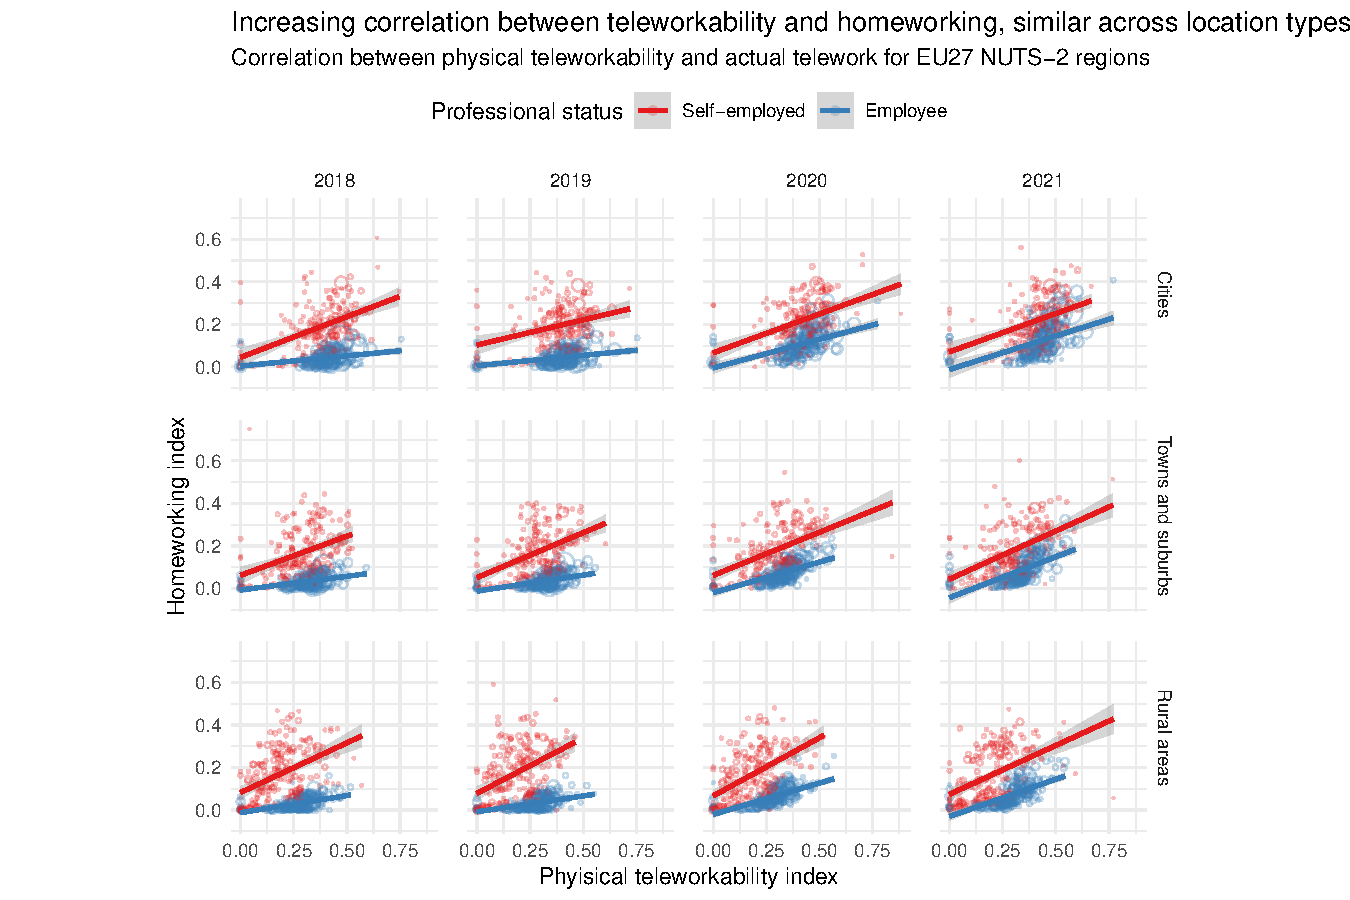
\includegraphics[width=\textwidth,height=0.9\textheight,keepaspectratio]{Correlation_teleworkability_telework_degurba.pdf}
\end{frame}


\begin{frame}{Changes in telework \emph{intensity}: cities vs rural areas}
\pause
\centering
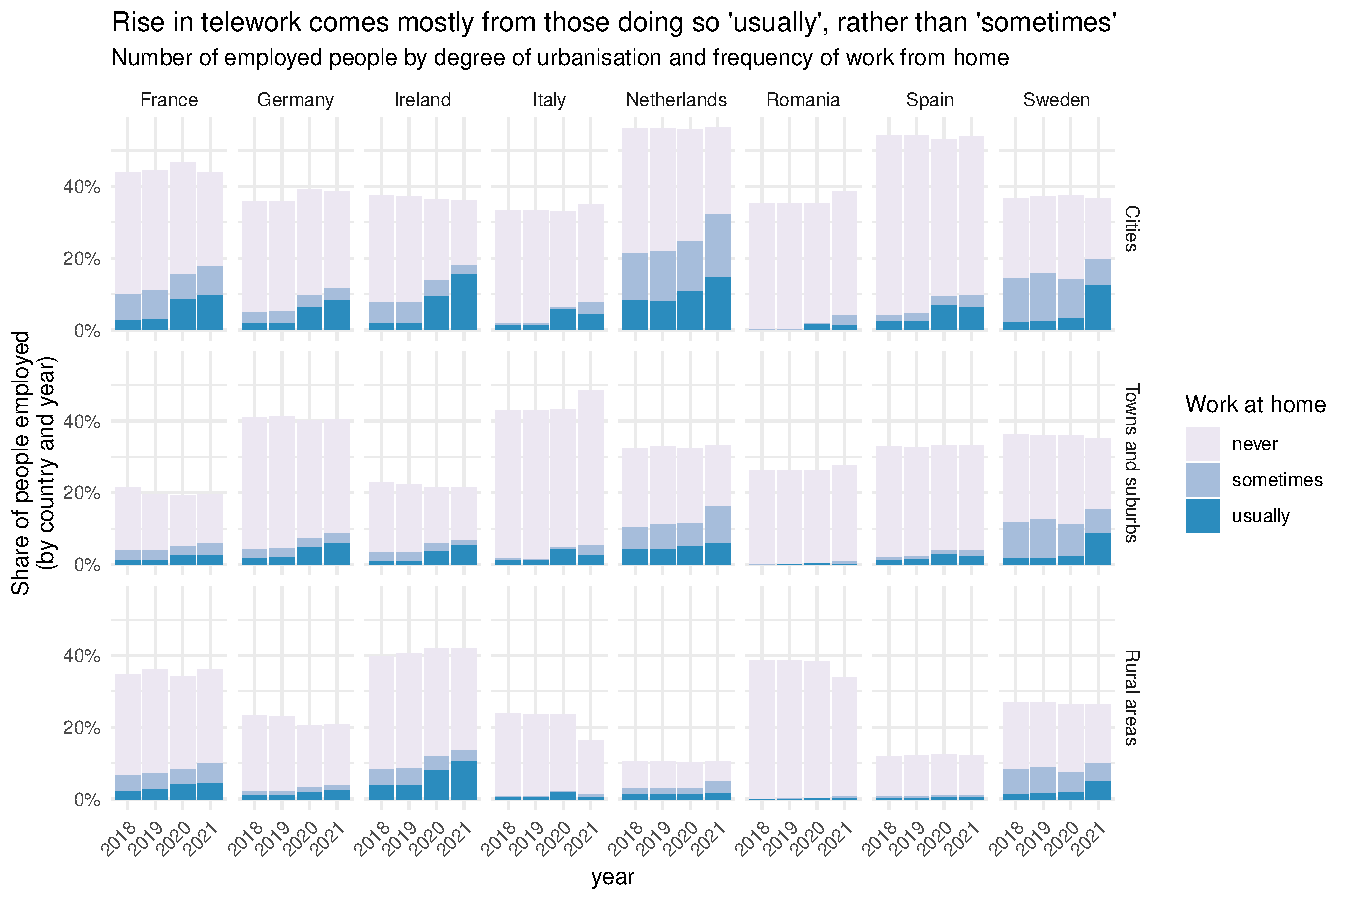
\includegraphics[width=\textwidth,height=0.9\textheight,keepaspectratio]{Telework_intensity_degurba_selected.pdf}
\end{frame}

\begin{frame}{Changes in telework \emph{intensity} in Ireland: cities vs rural areas}
\pause
\centering
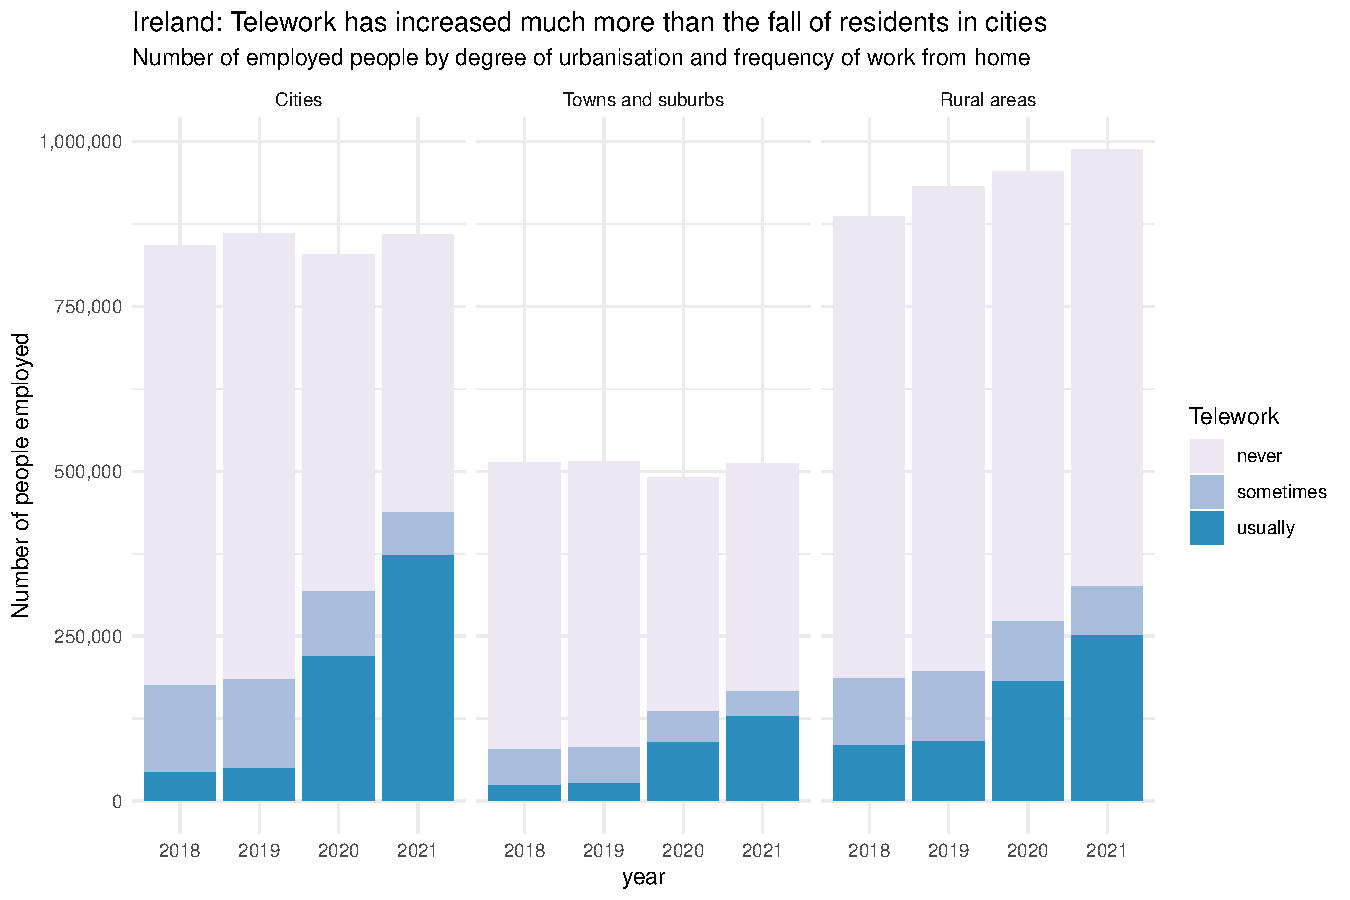
\includegraphics[width=\textwidth,height=0.9\textheight,keepaspectratio]{Telework_intensity_degurba_ireland.pdf}
\end{frame}


\begin{frame}{Change in telework index by degree of urbanisation}
Interpretation:
\begin{itemize}
\item Telework increased everywhere in 2020 (except Sweden, 2021)
\item De-coupling of cities from towns/suburbs and rural areas in 2020: how about capital cities?
\item Limited evidence of a trend before 2020
\item Similar trends over time across countries, but different absolute levels.
\item Surprising change in the \emph{extensive} margin in the aggregate (`never' $\Rightarrow$ `usually') rather than intensive margin (`never' $\Rightarrow$ `sometimes', or `sometimes' $\Rightarrow$ `usually')
\end{itemize}
\end{frame}

\section{Urban-rural region}
\begin{frame}{Telework index by urbrur}
\centering
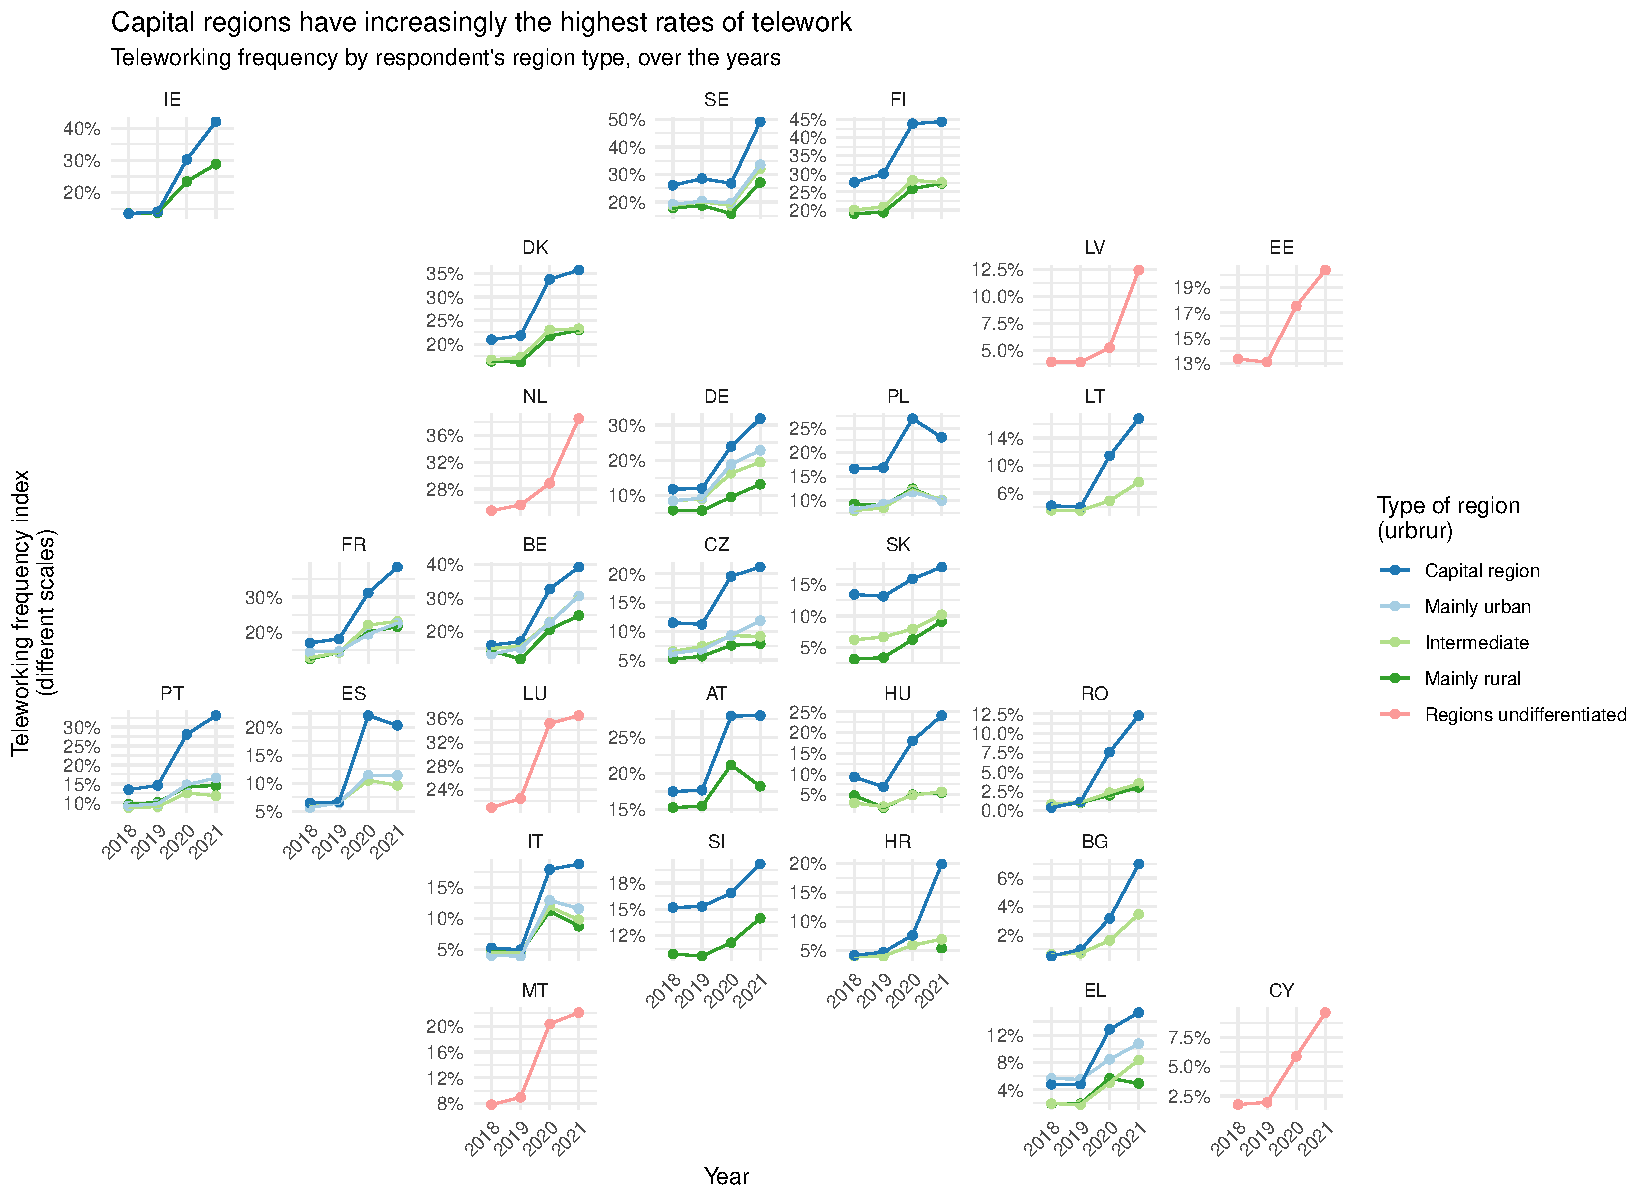
\includegraphics[width=\textwidth,height=0.9\textheight,keepaspectratio]{Telework_urbrur_eu.pdf}
\end{frame}

\begin{frame}{Changes in telework: cities vs rural areas}
\centering
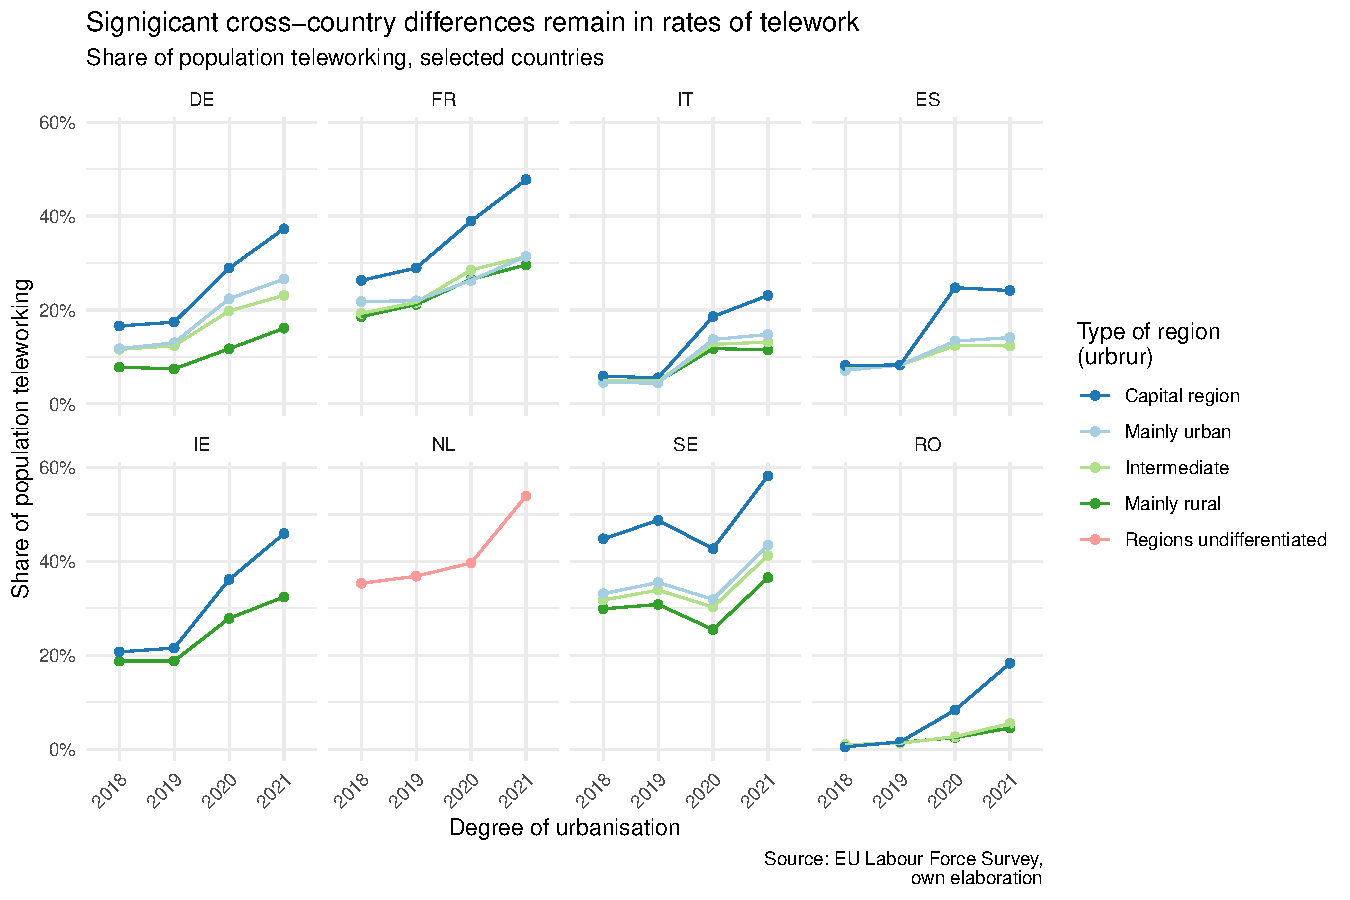
\includegraphics[width=\textwidth,height=0.9\textheight,keepaspectratio]{Telework_urbrur_selected.pdf}
\end{frame}


\begin{frame}{Change in telework index by urban-rural region}
Interpretation:
\begin{itemize}
\item Because urbrur is defined at the NUTS regional level, limited geographical granularity and coverage.
\item However, it shows a `capital city' premium (possibly in excess of over urban areas)
\end{itemize}
\end{frame}




\section{Regional internet connectivity statistics}

\begin{frame}{Access to internet by NUTS regions}
\centering
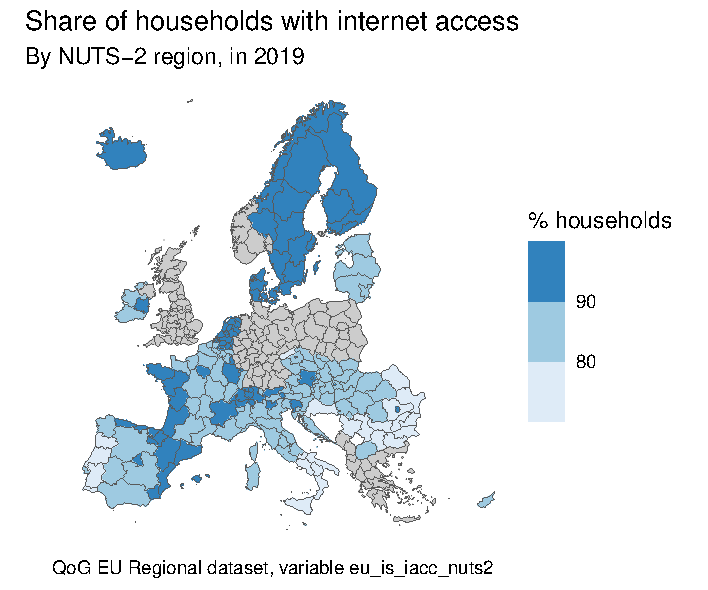
\includegraphics[width=\textwidth,height=0.9\textheight,keepaspectratio]{nuts_internet_2019.pdf}
\end{frame}

\begin{frame}{Access to internet by NUTS regions}
\centering
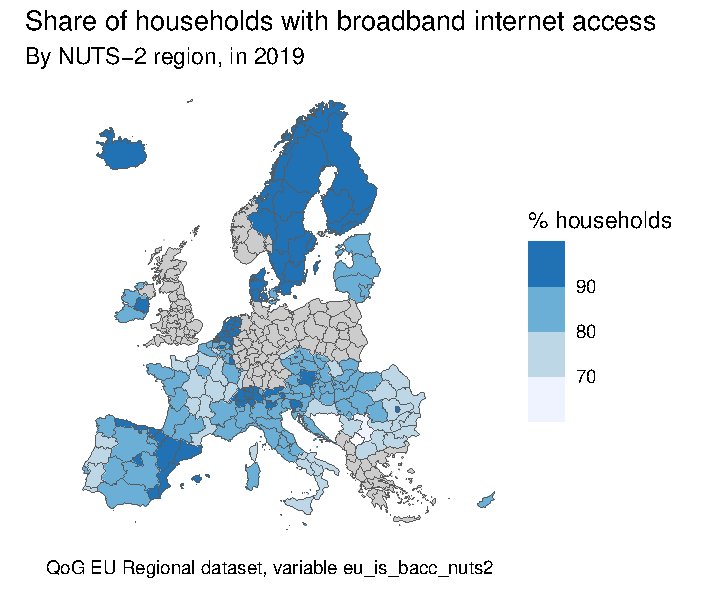
\includegraphics[width=\textwidth,height=0.9\textheight,keepaspectratio]{nuts_broadband_2019.pdf}
\end{frame}

\begin{frame}{Regional internet connectivity statistics}
Interpretation:
\begin{itemize}
\item Low coverage and geographical granularity from EU ICT survey.
\item Howver, JRC is working on regional statistics.
\end{itemize}
\end{frame}

\section{Occupational determinants of telework}

\begin{frame}{Teleworkability (ie, \emph{occupation}) is an increasingly good predictor of telework}
\pause
\centering
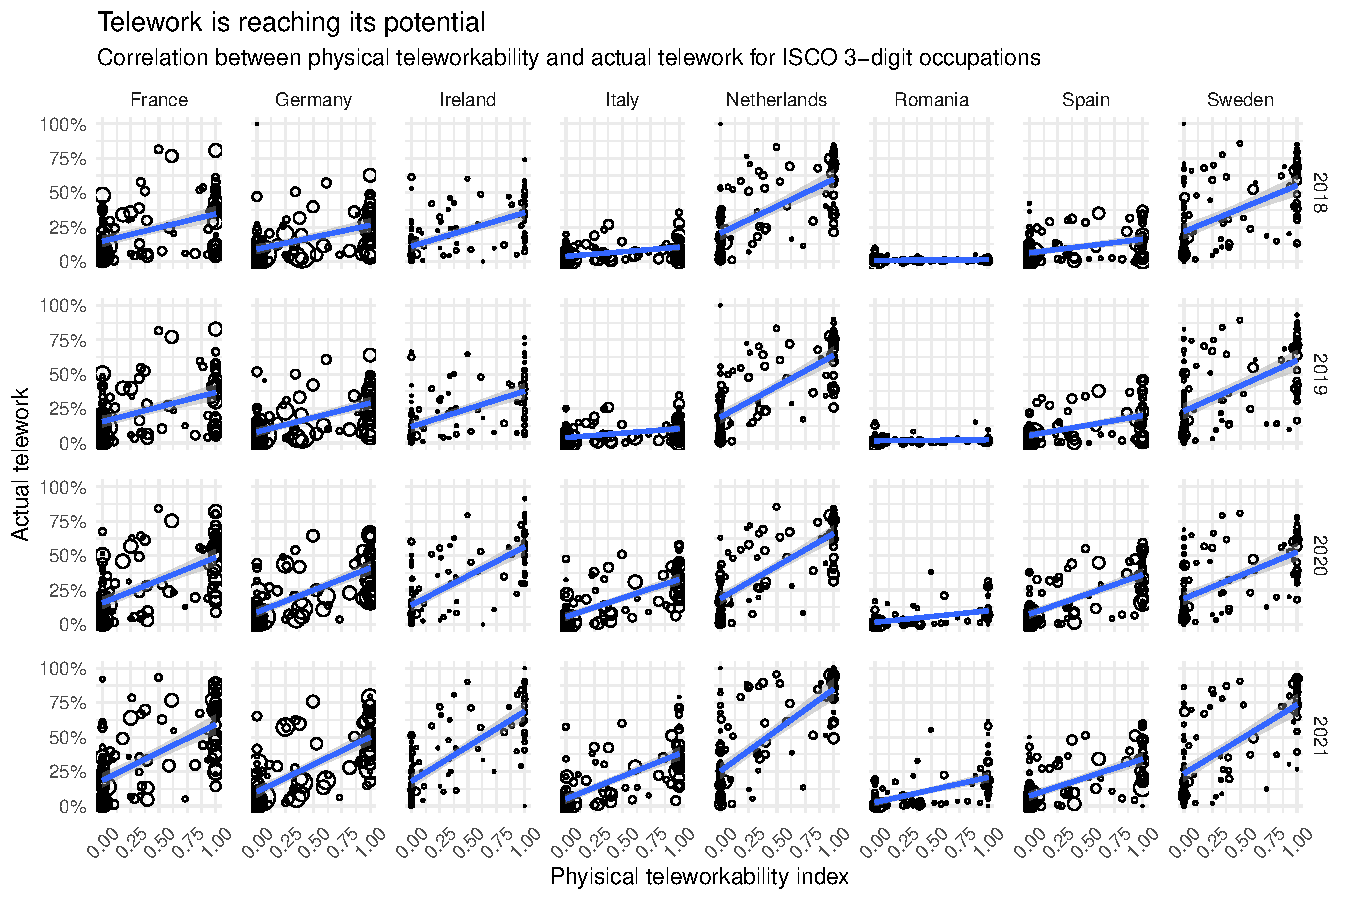
\includegraphics[width=\textwidth,height=0.9\textheight,keepaspectratio]{Correlation_teleworkability_telework_selected.pdf}
\end{frame}


\begin{frame}{Could telework ultimataly be down to (national/regional) employment structure?}
\pause
\centering
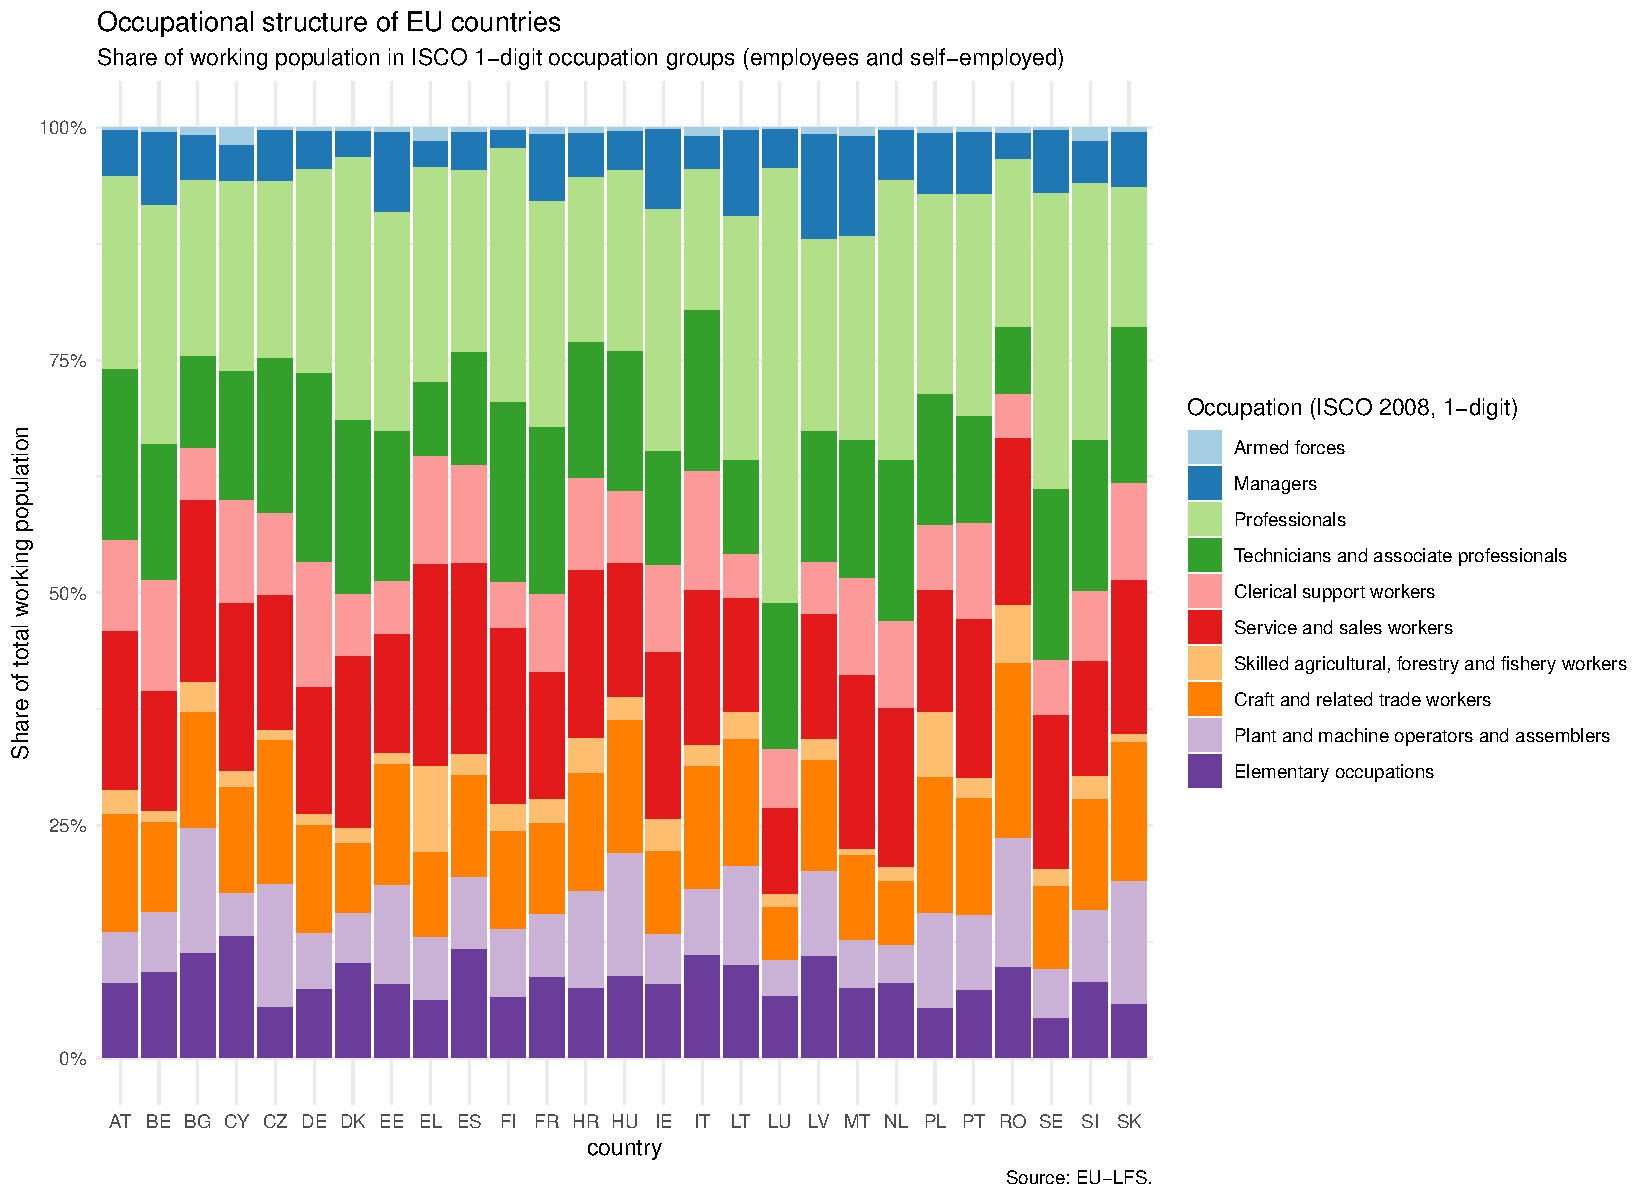
\includegraphics[width=\textwidth,height=0.9\textheight,keepaspectratio]{LFS_occup_structure.pdf}
\end{frame}


\begin{frame}{Variation in occupational rates of telework across countries}
\pause
\centering
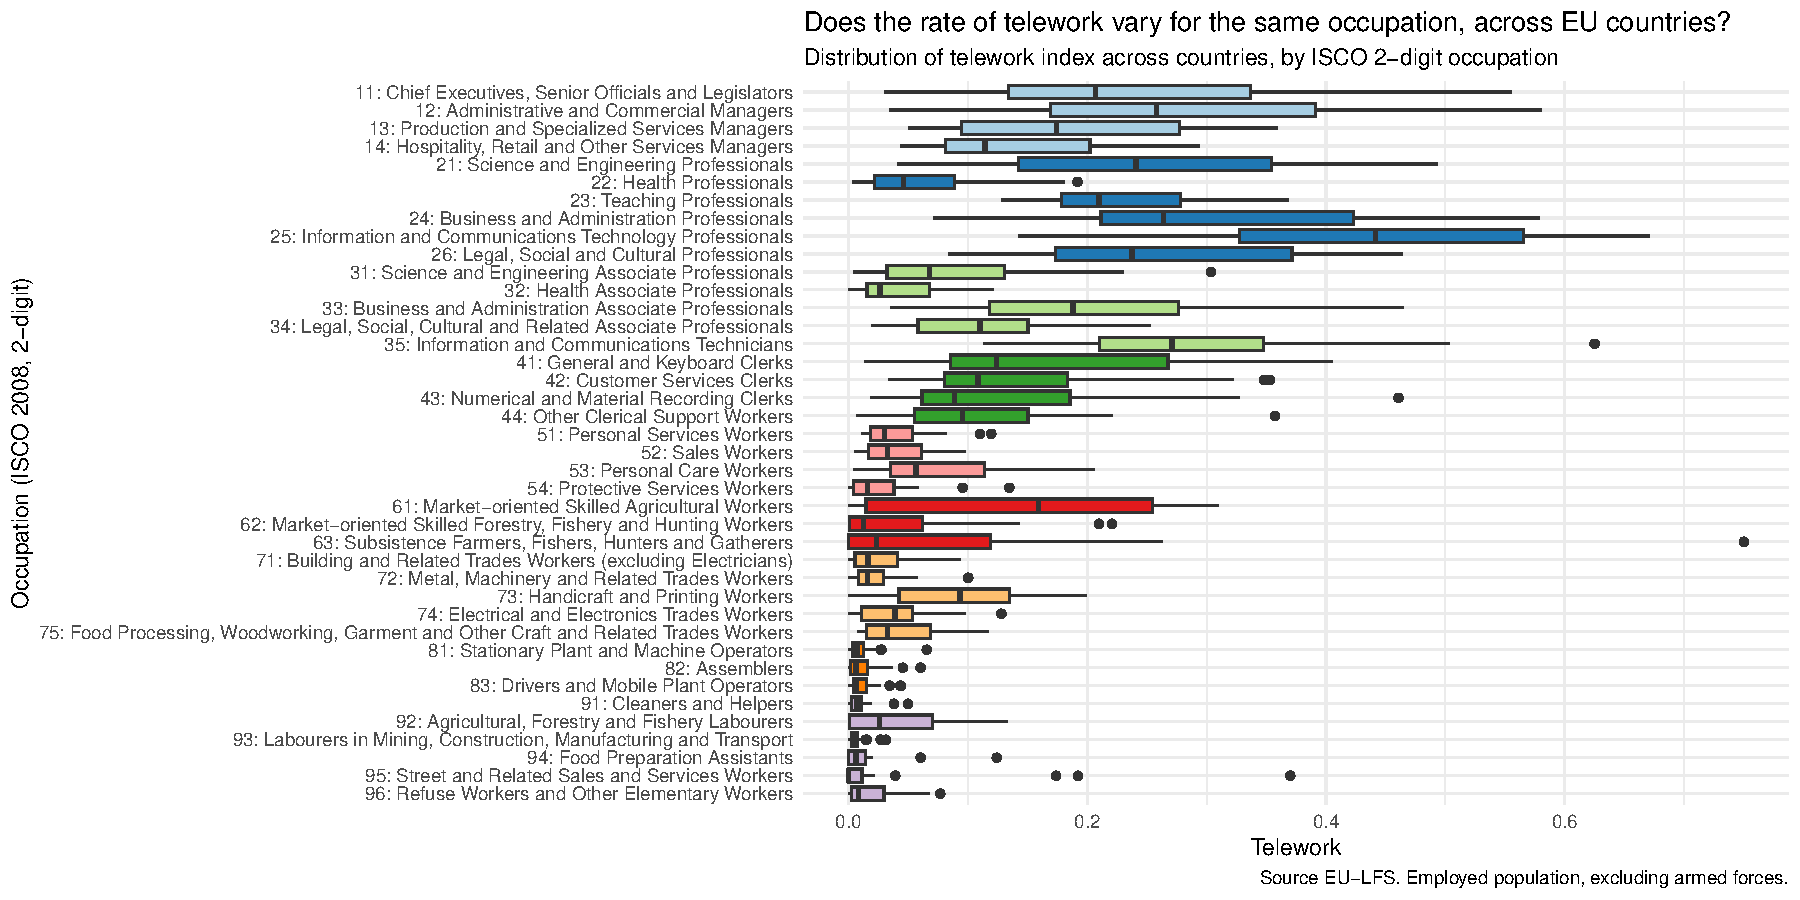
\includegraphics[width=\textwidth,height=0.9\textheight,keepaspectratio]{Variation_telework_occupation_boxplot.pdf}
\end{frame}

\begin{frame}{Variation rates of telework for specific occupation}
\pause
\centering
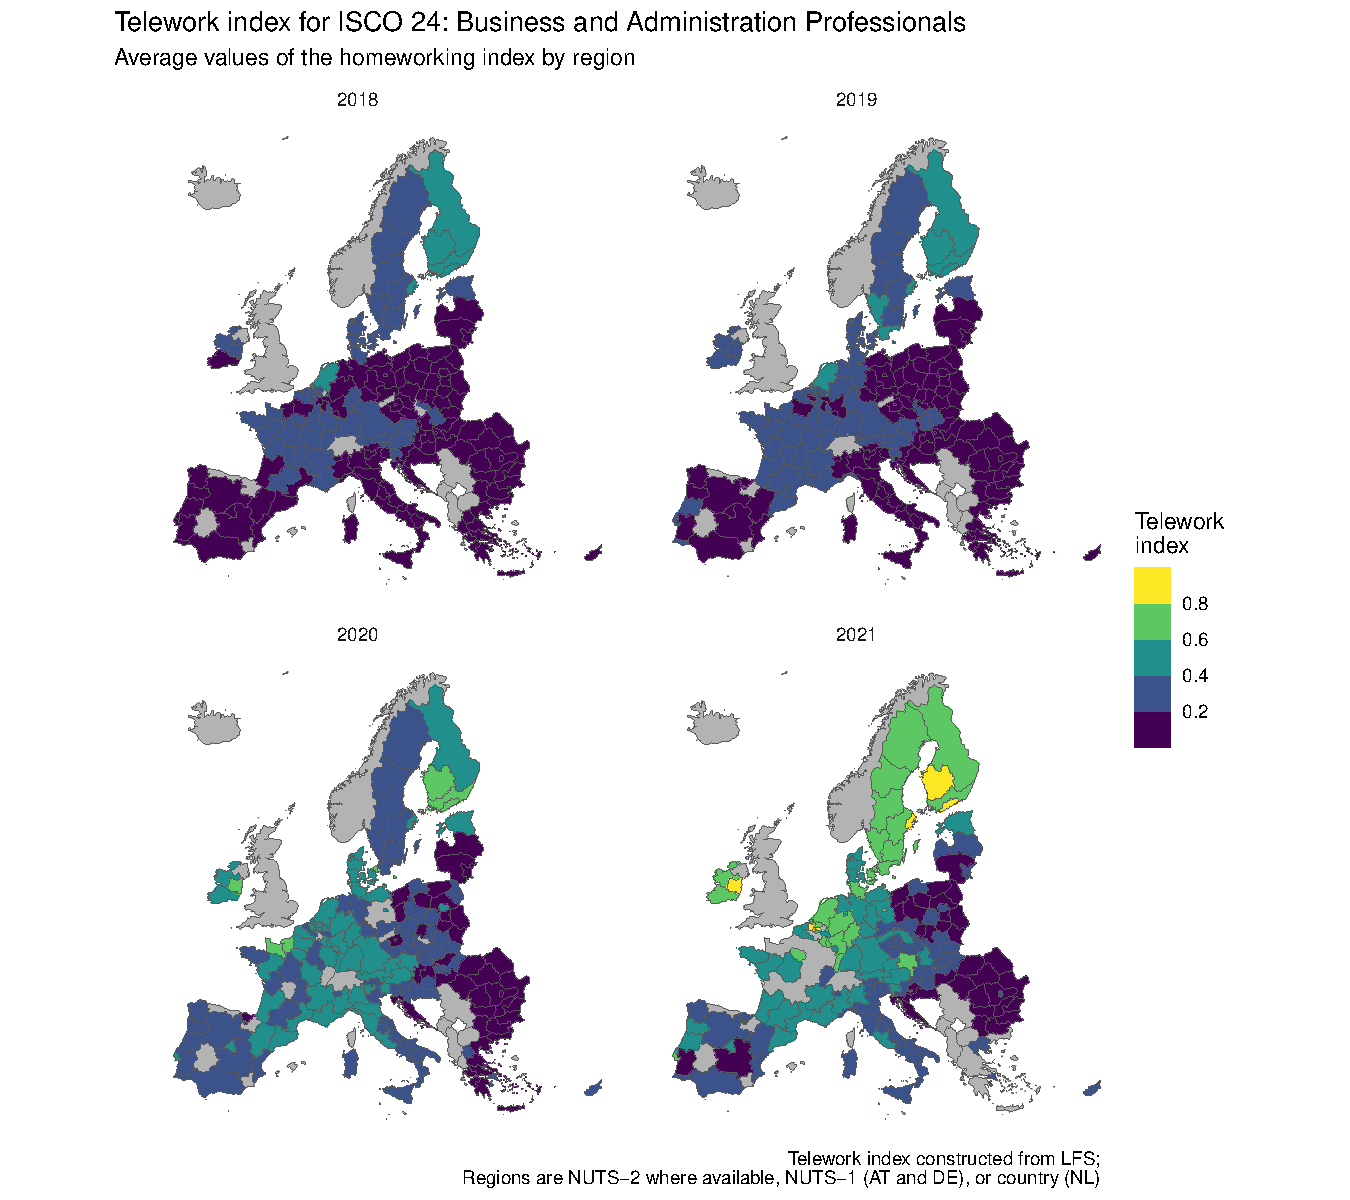
\includegraphics[width=\textwidth,height=0.9\textheight,keepaspectratio]{telework_isco24_countries.pdf}
\end{frame}




\section{Housekeeping}
\begin{frame}{Housekeeping}
\begin{itemize}
  \item LFS sample size over time, timing of survey in 2020.
  \item Sampling weight missing.
  \item Nomenclature:
    \begin{itemize}
      \item \emph{Telework}, \emph{Homeworking}, \emph{Working from home}?
      \item Degurba, urbrur?
    \end{itemize}
\end{itemize}
\end{frame}

\begin{frame}{LFS response rates}
\centering
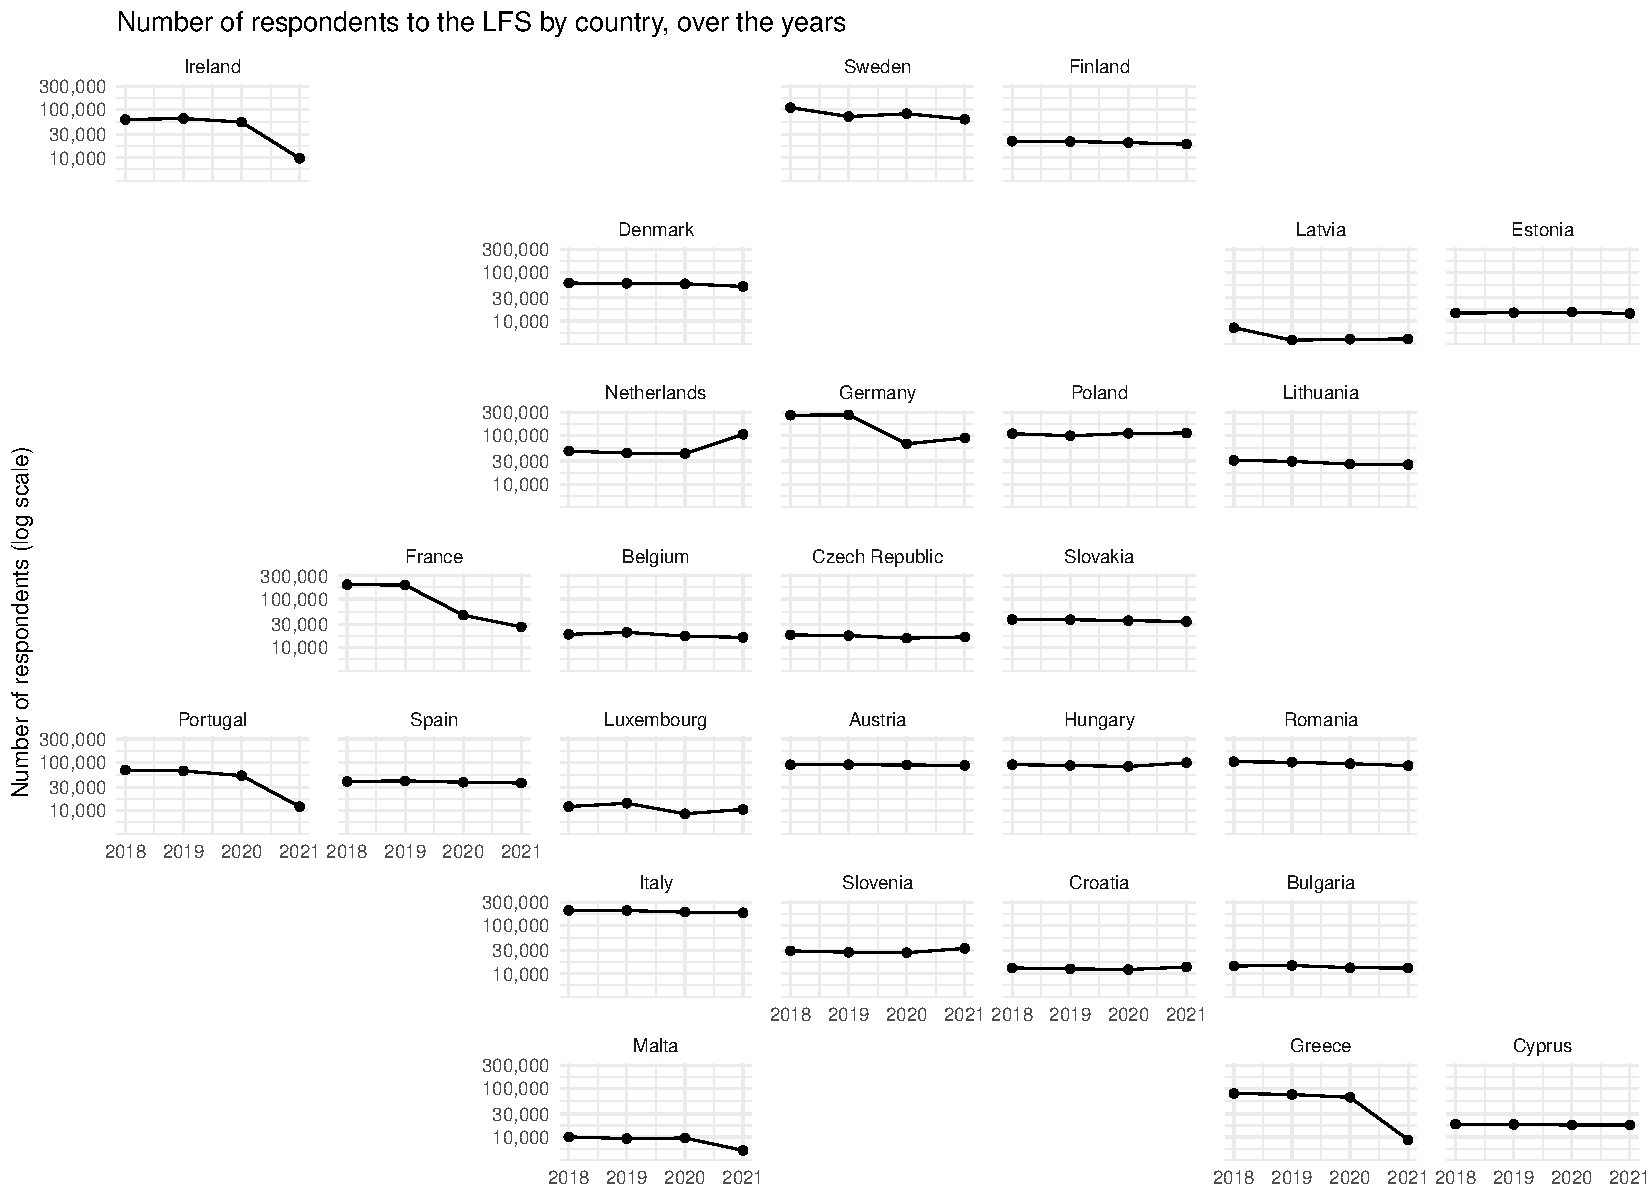
\includegraphics[width=\textwidth,height=0.9\textheight,keepaspectratio]{LFS_respondents_time.pdf}
\end{frame}


\begin{frame}{Share of observations with missing sampling weights (coeffy)}
\centering
\begin{table}[ht]
\centering
\begin{tabular}{lrrrr}
  \hline
  country & 2018 & 2019 & 2020 & 2021 \\ 
  \hline
  DK & 13.64 & 14.03 & 14.41 & 13.58 \\ 
  ES & 5.97 & 7.19 & 2.56 & 0.00 \\ 
  FI & 48.20 & 48.01 & 47.27 & 45.69 \\ 
  LU & 0.00 & 0.00 & 0.00 & 49.69 \\ 
  LV & 43.47 & 0.00 & 0.00 & 0.00 \\ 
  NL & 0.00 & 0.00 & 0.00 & 55.61 \\ 
  SE & 2.53 & 3.39 & 3.63 & 4.74 \\ 
  \hline
\end{tabular}
\end{table}
\end{frame}



\begin{frame}{Takeaways}

\begin{enumerate}
\item Marked changes in overall telework frequency (as measured from LFS) relative to before COVID
\item Significant variation \emph{across} countries (country fixed-effect).
\item Variation \emph{within} countries, in terms of urban areas vs the rest.
\item Capital city premium, worth adding as additional control on top of degurba.
\item Changing telework intensity: surprising change in the \emph{extensive} margin in the aggregate (`never' $\Rightarrow$ `usually') rather than intensive margin (`never' $\Rightarrow$ `sometimes', or `sometimes' $\Rightarrow$ `usually')
\item Ireland as an extreme case.
\item Circumstantial evidence of limited relocation for telework.
\end{enumerate}

\end{frame}

\begin{frame}{Explanations/mechanisms}
Explanations:
\begin{itemize}
  \item Occupational structure (across an within countries);
  \item National-level institutions, corporate culture, industrial structure;
  \item Regional connectivity?
  \item Cost of housing?
\end{itemize}
\end{frame}


\end{document}
